\documentclass[12pt,a4paper,titlepage]{report}
\usepackage[english]{babel}
\usepackage[utf8]{inputenc}
\usepackage{xcolor}
\usepackage{graphicx}
\usepackage{subcaption}
\graphicspath{ {./images/} }
\usepackage[font=small,labelfont=bf]{caption}
\usepackage{listings}
\usepackage{amsmath}
\usepackage{amssymb}
\usepackage[round]{natbib}
\bibliographystyle{apalike}
\usepackage{setspace}
\usepackage{etoolbox}
\AtBeginEnvironment{quote}{\par\singlespacing\small}
\usepackage[top=50pt,bottom=50pt,left=60pt,right=60pt]{geometry}

\usepackage{enumitem}
\usepackage{hyperref}
\usepackage[noabbrev]{cleveref}


\pagestyle{headings}

\hypersetup{
    colorlinks=true,
    linkcolor=black,
    citecolor=black,
    urlcolor=blue,
}


\newcommand*\ttvar[1]{\texttt{\expandafter\dottvar\detokenize{#1}\relax}}
\newcommand*\dottvar[1]{\ifx\relax#1\else
  \expandafter\ifx\string_#1\string_\allowbreak\else#1\fi
  \expandafter\dottvar\fi}

\definecolor{codegreen}{rgb}{0,0.6,0}
\definecolor{codegray}{rgb}{0.5,0.5,0.5}
\definecolor{codepurple}{rgb}{0.58,0,0.82}
\definecolor{backcolour}{rgb}{0.95,0.95,0.92}

\lstdefinestyle{mystyle}{
    backgroundcolor=\color{backcolour},   
    commentstyle=\color{codegreen},
    keywordstyle=\color{magenta},
    numberstyle=\tiny\color{codegray},
    stringstyle=\color{codepurple},
    basicstyle=\ttfamily\footnotesize,
    breakatwhitespace=false,         
    breaklines=true,                 
    captionpos=b,                    
    keepspaces=true,                 
    numbers=left,                    
    numbersep=5pt,                  
    showspaces=false,                
    showstringspaces=false,
    showtabs=false,                  
    tabsize=2
}

\lstset{style=mystyle}



\newcommand{\what}[1] {\textcolor{red}{#1}}

\newcommand{\todo}[1] {\textcolor{orange}{\textbf{TODO: #1} \addcontentsline{toc}{subsection}{\textcolor{orange}{TODO: #1}}
}}

\newcommand{\image}[3][1]
{
\begin{figure}
	\centerline{\includegraphics[width={1\linewidth}]{#1}}
	\caption{#2}
	\label{#3}
\end{figure}
}



\begin{document}

\title{Learning in cortical microcircuits with multi-compartment pyramidal neurons}
\author{Johannes Gille}
\date{\parbox{\linewidth}{\centering%
Thesis notes
\endgraf
  \today\endgraf\bigskip
  M.Sc. Kognitive und integrative Systemneurowissenschaften\medskip\endgraf
  Philipps-Universität Marburg\endgraf
  \bigskip
  \bigskip
  \textbf{Supervisors:}\endgraf
  \bigskip
  Prof. Dr. Dominik Endres, Philipps-Universität Marburg\endgraf
  \bigskip
  Dr. Johan Kwisthout, Radboud University}}
\maketitle




\section{utilities}

One-sided exponential decay kernel

\begin{align}
\kappa(t) &= H(t)e^{-t/\tau_{\kappa}} \\
H(t) &= 
	\begin{cases}
		1 & \text{if $t > 0$}\\
		0 & \text{if $t \leq 0$}\\
	\end{cases}
\end{align}

Antiderivatives:

\begin{align}
\int_{-\infty}^x H(t)dt = tH(t) = max(0,t)
\end{align}

Convolution:

\begin{align*}
(f \ast g)(t) &= \int_{- \infty }^{\infty} f(\tau) g(t-\tau) d \tau
\end{align*}
For functions f, g supported on only $[0, \infty]$ (as one-sided decay kernels and spiketrains are), integration limits can be truncated:
\begin{align*}
(f \ast g)(t) &= \int_{0}^{t} f(\tau) g(t-\tau) d \tau\\
\end{align*}


Plasticity:

\begin{align}
\frac{dW_{ij}}{dt}(t)&= F(W_{ij}(t), s_i^\ast (t), s_j^\ast (t), V_i^\ast (t))\\
F[s_j^\ast, V_i^\ast] &= \eta \kappa \ast (V_i^\ast s_j^\ast)\\
\text{with } V_i^\ast &= (s_i - \phi(V_i )) h(V_i),\\
s_j^\ast &= \kappa_s \ast s_j.
\end{align}

For an event-based plasticity we need:

\begin{align}
\Delta W_{ij}(t,T) &= \int_t^T dt' F[s_j^\ast , V_i^\ast ](t')\\
 &= \int_t^T dt' \eta \kappa \ast (V_i^\ast s_j^\ast)\\
 &= \eta \int_t^T dt' \  \int_0^{t'} dt'' \ \kappa(t'-t'') V_i^\ast (t'') s_j^\ast (t'')\\
 &= \eta \int_0^t dt' \  \int_{t''}^{t'} dt'' \ \kappa(t'-t'') V_i^\ast (t'') s_j^\ast (t'')\\
\end{align}


Starting with the complete Integral from $t=0$.

\begin{align*}
\Delta W_{ij}(0,t) &=\eta \int_0^t dt' \  \int_0^{t'} dt'' \ \kappa(t'-t'') V_i^\ast (t'') s_j^\ast (t'')\\
 &= \eta \int_0^t dt'' \  \int_{t''}^{t} dt' \ \kappa(t'-t'') V_i^\ast (t'') s_j^\ast (t'')\\
  &= \eta \int_0^t dt'' \  \left[ \tilde{\kappa}(t-t'') - \tilde{\kappa}(0) \right] V_i^\ast (t'') s_j^\ast (t'')\\
\end{align*}

With $\tilde{\kappa}$ being the antiderivative of $\kappa$: 

\begin{align*}
\kappa(t) &= \frac{\delta}{\delta t} \tilde{\kappa}(t)\\
\tilde{\kappa}(t) &= - e^{-\frac{t}{t_{\kappa}}} \\
\end{align*}

The above can be split up into two separate integrals:
\begin{align*}
\Delta W_{ij}(0,t) &=\eta \left[ -I_2 (0, t) + I_1(0,t) \right] \\
I_1(t_1, t_2) &= - \int_{t_1}^{t_2} dt' \ \tilde{\kappa} (0) V_i^\ast (t') s_j^\ast (t')\\
I_2(t_1, t_2) &= - \int_{t_1}^{t_2} dt' \ \tilde{\kappa} (t_2 - t') V_i^\ast (t') s_j^\ast (t')\\
\end{align*}

Which implies the identities 

\begin{align*}
I_1(t_1, t_2 + \Delta t) &= I_1 (t_1, t_2) + I_1 (t_2, t_2 + \Delta t)\\
I_2(t_1, t_2 + \Delta t) &= e^{- \frac{t_2 - t_1}{\tau_{\kappa}}} I_2 (t_1, t_2) + I_2 (t_2, t_2 + \Delta t)
\end{align*}


\begin{align}
I_2 (t_1, t_2 + \Delta t) &= -\int_{t_1}^{t_2 + \Delta t} dt' \ \tilde{\kappa} (t_2 + \Delta t - t') V_i^\ast (t') s_j^\ast (t')\\
&= -\int_{t_1}^{t_2} dt' \ \left[ -e^{- \frac{t_2 + \Delta t - t'}{\tau_\kappa}} \right] V_i^\ast (t') s_j^\ast (t') 
 -\int_{t_2}^{t_2 + \Delta t} dt' \ \left[ -e^{- \frac{t_2 + \Delta t - t'}{\tau_\kappa}} \right] V_i^\ast (t') s_j^\ast (t')\\
 &= -e^{- \frac{ \Delta t}{\tau_\kappa}} \int_{t_1}^{t_2} dt' \ \left[ -e^{- \frac{t_2 - t'}{\tau_\kappa}} \right] V_i^\ast (t') s_j^\ast (t') 
 -\int_{t_2}^{t_2 + \Delta t} dt' \ \left[ -e^{- \frac{t_2 + \Delta t - t'}{\tau_\kappa}} \right] V_i^\ast (t') s_j^\ast (t')
\end{align}


Using this we can rewrite the weight change from $t$ to $T$ as:


\begin{align*}
\Delta W_{ij}(t,T) &= \Delta W_{ij}(0,T) - \Delta W_{ij}(0,t)\\
&= \eta [-I_2(0,T) + I_1(0,T) + I_2(0,t) - I_1(0,t)]\\
&= \eta [I_1(t,T) - I_2(t,T) + I_2(0,t)\left( 1 - e^{- \frac{T-t}{\tau_\kappa}} \right)]
\end{align*}

The simplified \cite{sacramento2018dendritic} case would be:

\begin{align*}
\frac{dW_{ij}}{dt} &= \eta (\phi(u_i) - \phi(\hat{v_i})) \phi(u_j)\\
\Delta W_{ij}(t,T) &= \int_t^T dt' \ \eta \  (\phi(u_i^{t'}) - \phi(\widehat{v_i^{t'}})) \  \phi(u_j^{t'})\\
\Delta W_{ij}(t,T) &= \eta \int_t^T dt' \  (\phi(u_i^{t'}) - \phi(\widehat{v_i^{t'}})) \ \phi(u_j^{t'})\\
V_i^* &= \phi(u_i^{t'}) - \phi(\widehat{v_i^{t'}})\\
s_j^* &= \kappa_s * s_j
\end{align*}


Where $s_i$ is the postsynaptic spiketrain and $V_i^*$ is the error between dendritic prediction and somatic rate and $h( u )$. The additional nonlinearity $h( u ) = \frac{d}{du} ln \  \phi(u)$ is ommited in our model \todo{should it though?}.



\begin{align}
\tau_l &= \frac{C_m}{g_L} = 10\\
\tau_s &= 3
\end{align}

Writing membrane potential to history (happens at every update step of the postsynaptic neuron:

\begin{lstlisting}[language=C++, directivestyle={\color{black}}
                   emph={int,char,double,float,unsigned,exp},
                   emphstyle={\color{blue}}]

UrbanczikArchivingNode< urbanczik_parameters >::write_urbanczik_history(Time t, double V_W, int n_spikes, int comp)
{
	double V_W_star = ( ( E_L * g_L + V_W * g_D ) / ( g_D + g_L ) );
	double dPI = ( n_spikes - phi( V_W_star ) * Time::get_resolution().get_ms() )
      * h( V_W_star );
}\end{lstlisting}

I interpret this as:


\begin{align*}
\int_{t_{ls}}^T dt' \ V_i^* &= \int_{t_{ls}}^T dt' \  (s_i - \phi(V_i )) h(V_i),\\
\int_{t_{ls}}^T dt' \ V_i^* &= \sum_{t=t_{ls}}^T \  (s_i(t) -  \phi(V_i^t ) \Delta t) h(V_i^t)\\
\end{align*}

\begin{lstlisting}[language=C++, directivestyle={\color{black}}
                   emph={int,char,double,float,unsigned,exp},
                   emphstyle={\color{blue}}]
for (t = t_ls; t< T; t = t + delta_t)
{
   	minus_delta_t = t_ls - t;
    minus_t_down = t - T;
    PI = ( kappa_l * exp( minus_delta_t / tau_L ) - kappa_s * exp( minus_delta_t / tau_s ) ) * V_star(t);
    PI_integral_ += PI;
    dPI_exp_integral += exp( minus_t_down / tau_Delta_ ) * PI;
}  
// I_2 (t,T) = I_2(0,t) * exp(-(T-t)/tau) + I_2(t,T)
PI_exp_integral_ = (exp((t_ls-T)/tau_Delta_) * PI_exp_integral_ + dPI_exp_integral);
W_ji = PI_integral_ - PI_exp_integral_;
W_ji = init_weight_ + W_ji * 15.0 * C_m * tau_s * eta_ / ( g_L * ( tau_L - tau_s ) );    
  
kappa_l = kappa_l * exp((t_ls - T)/tau_L) + 1.0;
kappa_s = kappa_s * exp((t_ls - T)/tau_s) + 1.0;
  \end{lstlisting}


\begin{align*}
\int_{t_{ls}}^T dt' s_j^* &=  \tilde{\kappa_L}(t') * s_j -  \tilde{\kappa_s}(t') * s_j
\end{align*}

$I_1$ in the code is computed as a sum:

\begin{align}
I_1 (t,T) = \sum_{t'=t}^T \ (s_L^*(t') - s_s^*(t')) * V^*(t') 
\end{align}


\section{steady-state potentials in Sacramento (2018)}

\begin{align*}
u_k^p &= \frac{g_B}{g_{lk} + g_B + g_A} v^P_{B,k} + \frac{g_A}{g_{lk} + g_B + g_A} v^P_{A,k} \\
\hat{v}^P_{B,k} &= \frac{g_B}{g_{lk} + g_B + g_A} v^P_{B,k}\\
\hat{v}^I_{k} &= \frac{g_B}{g_{lk} + g_B} v^I_{k}\\
\lambda &= \frac{g_{som}}{g_{lk} + g_B + g_{som}}
\end{align*}



\begin{enumerate}
  \item In the torch implementation, there no persistence between timesteps at all. Input is fed into the network and processed feedforward and feedback. Output is read and weights (+biases) are updated. Rinse and repeat.
  \item to what extent should dendritic and somatic compartments decay?
  \item Can (should) we transfer the learned bias from the torch model?
  \item I can "cheat" the apical voltage constraint for self prediction by increasing apical leakage conductance. How does this influence my model?
  \item Is there some analytical approach to identifying why synaptic weights deviate from their intended targets?
  \item I think that lambda needs to be scaled in dependence on $g_{lk}$, such that current inputs, spike inputs and leakage cancel each other out.

    \item How do we deal with population size dependence?

\end{enumerate}

\section{Parameter study}
\begin{itemize}

 \item Transfer function $\phi$
 \item interneuron mixing factor $\lambda$
 \item injected current $I_e$
 \item dendritic leakage conductance $g_{lk,d}$
 \item somatic leakage conductance $g_{lk,s}$
 \item Learning rate $\eta$
 \item synaptic time constants $\tau_{delta}$
 \item noise level $\sigma$
 \item Simulation time $\mathbb{T}$
 \item plasticity onset after the network relaxes
 \item compartment current decay $\tau_{syn}$

\end{itemize}



\begin{figure}
	\centerline{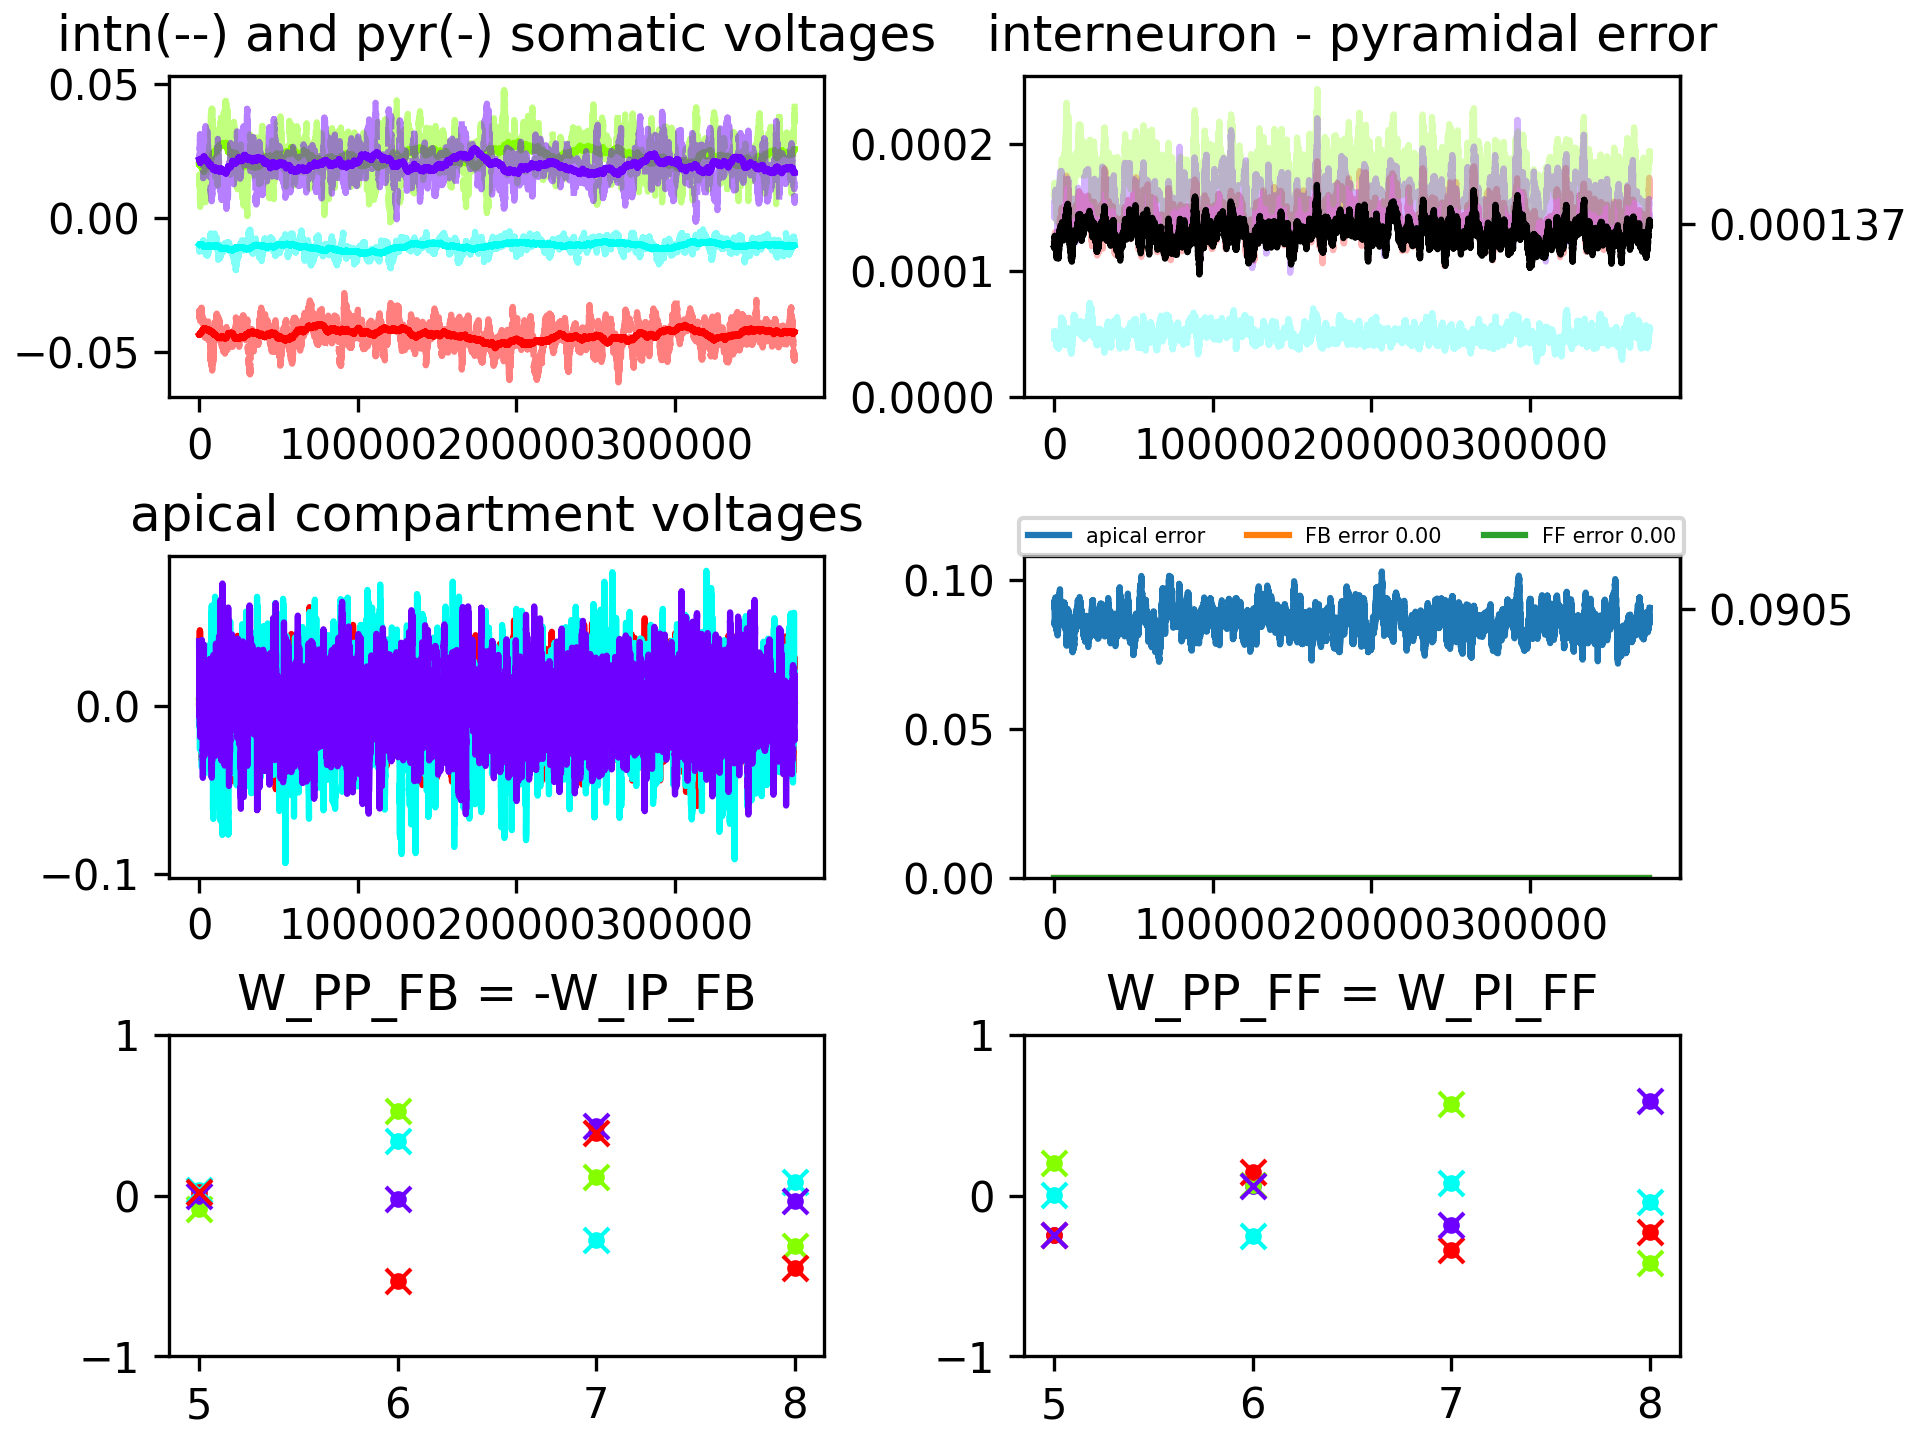
\includegraphics[width={1\linewidth}]{self_pred_static.png}}
	\caption{Self-predicting initialization without plasticity}
\end{figure}

\begin{figure}
	\centerline{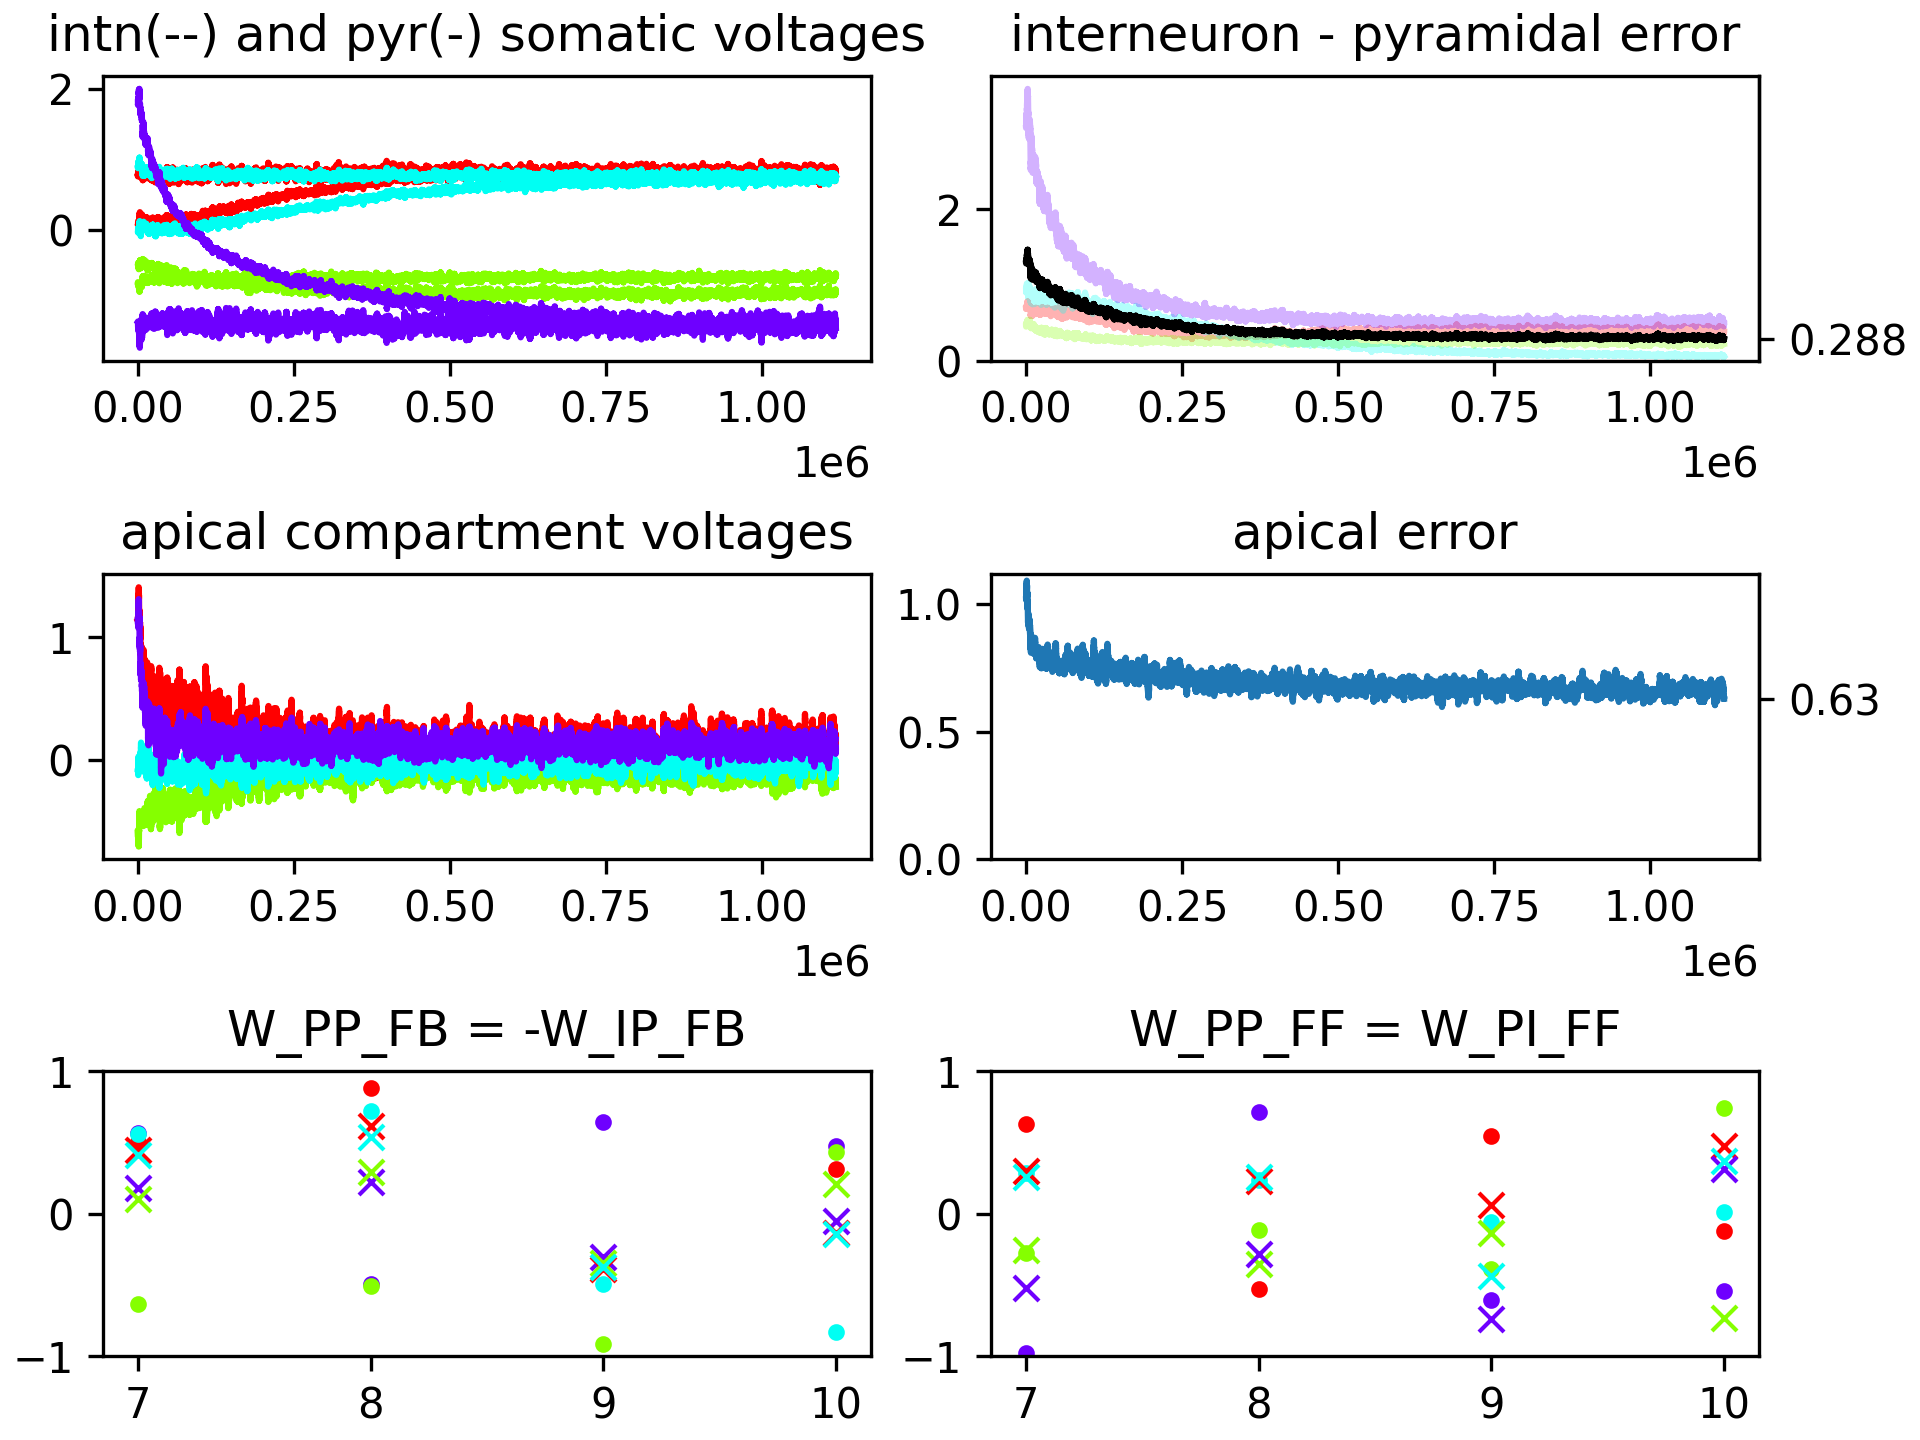
\includegraphics[width={1\linewidth}]{random_plastic.png}}
	\caption{Random initialization with plasticity enabled}
\end{figure}

\begin{figure}
	\centerline{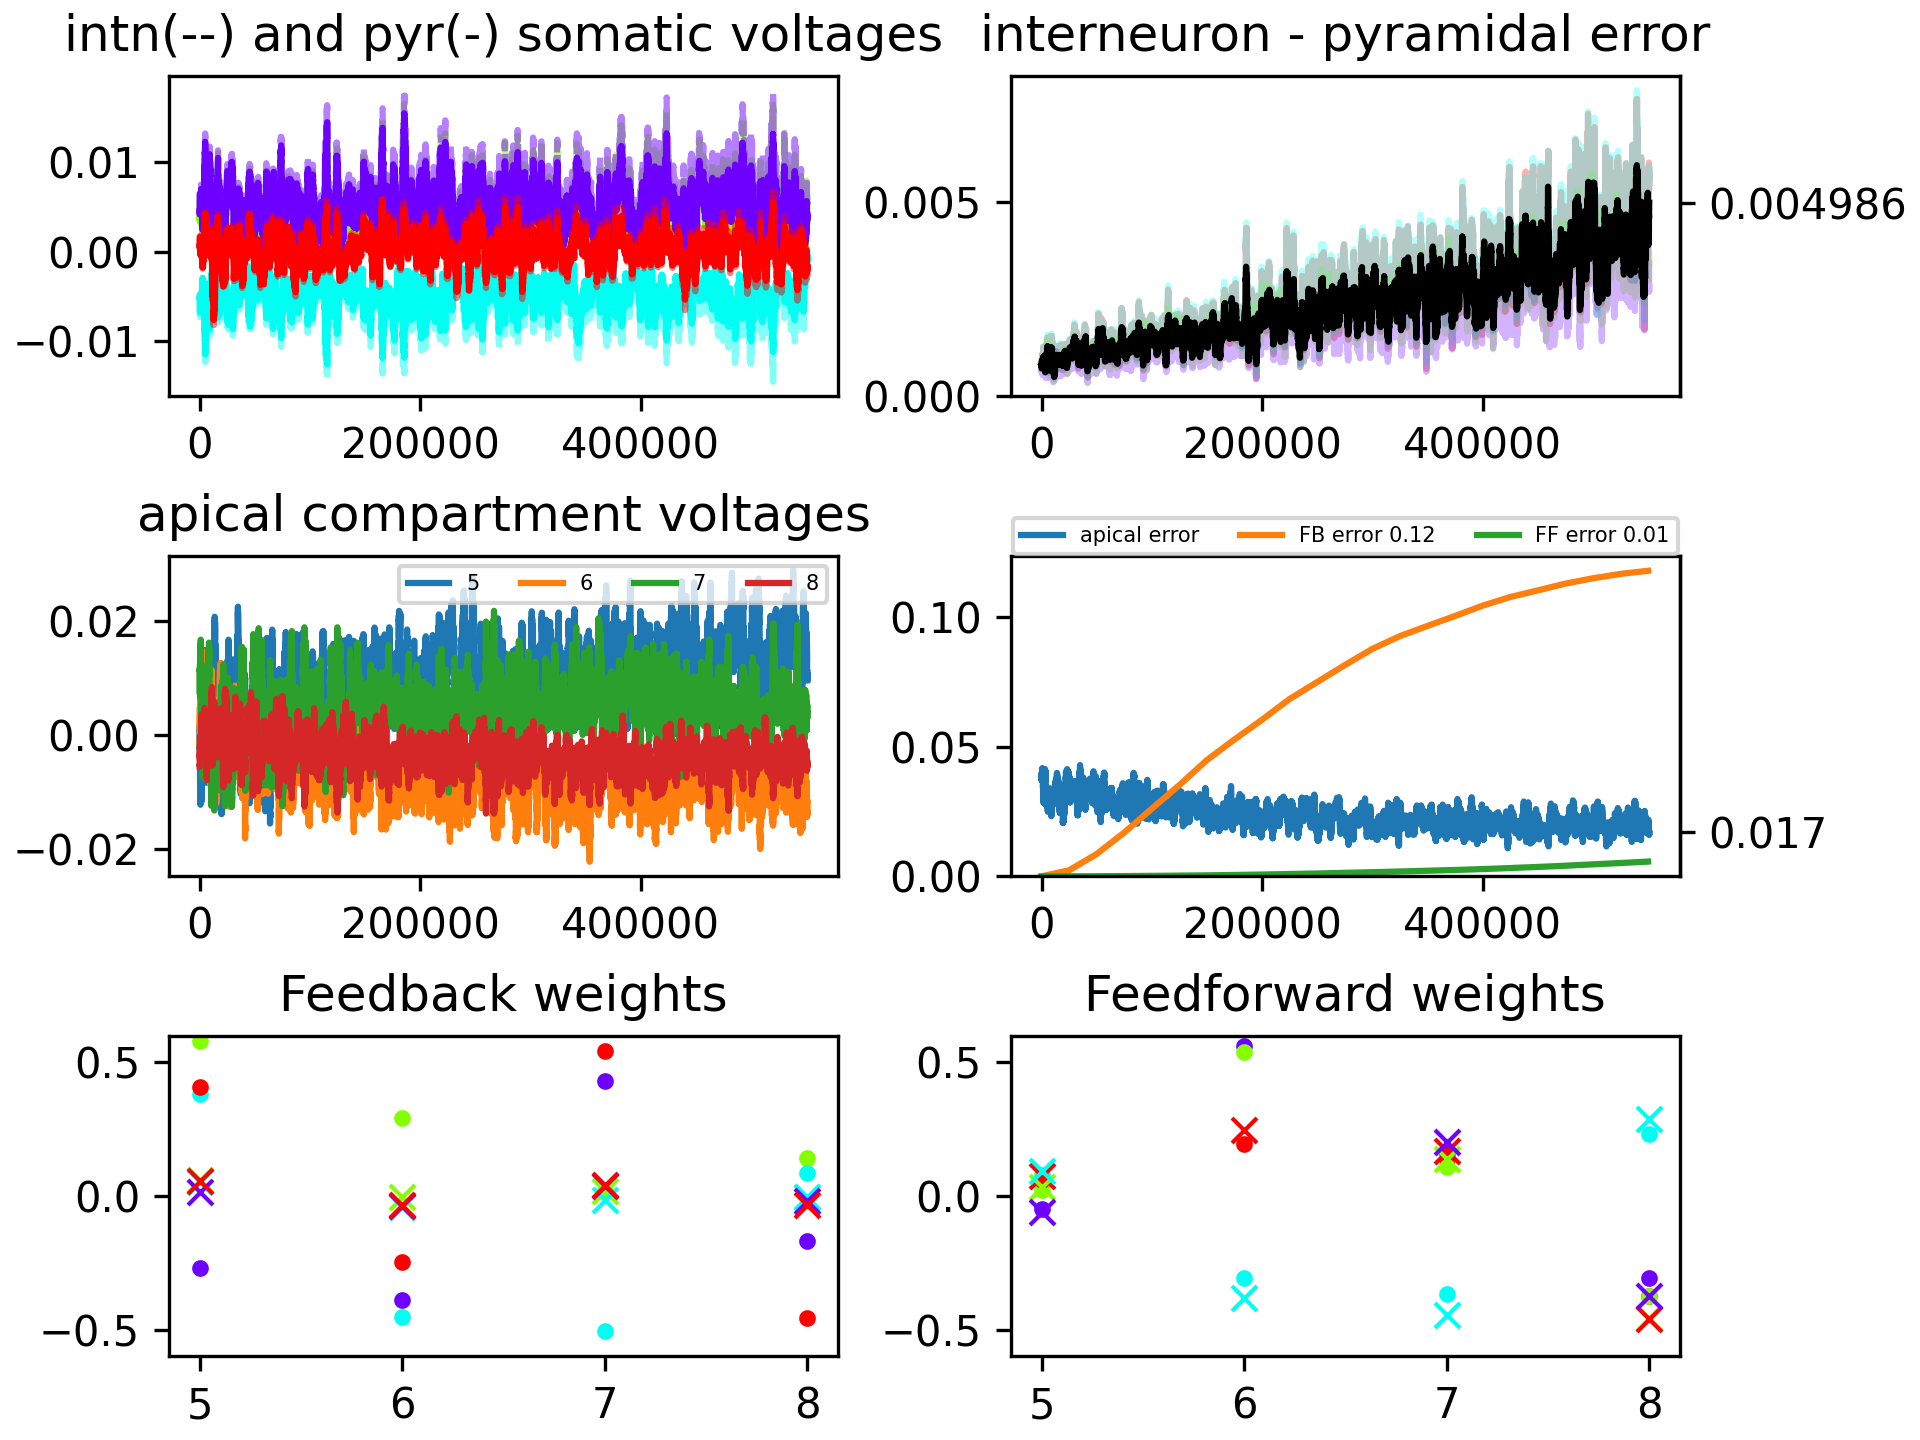
\includegraphics[width={1\linewidth}]{weird.png}}
	\caption{Self-predicting initialization with plasticity enabled. Feedback weights collapse pretty quickly; feedforward weights remain shockingly stable. This seems to be neuron-specific. In other simulations of equal parametrization, only 1/4 remained stable compared to 3/4 as seen here. Apical voltage decreases over time, which somehow makes sense as feedback int$\rightarrow$pyr weights are reduced to zero. Yet these would ideally precisely counteract feedback pyr weights.}
\end{figure}


\subsection*{Observations}

\begin{itemize}
\item In self-predicting paradigm, Apical errors stay constant, despite interneuron error steadily increasing.
\item Interneuron error (between neuron pairs) is proportional to absolute somatic voltage in self-predicting paradigm.
\item abs interneuron voltage is always higher than abs pyramidal voltage. This kind of makes sense, as interneurons receive direct current input proportional to pyramidal voltage in addition to feedforward input. This discrepancy disappears when setting $\lambda$ to 0 as expected.
\item When plasticity is enabled from a random starting configuration, apical error \textbf{sometimes} converges to better values than can be achieved in both self-predicting paradigms. I believe this to be a huge issue: the self-predicting state does not cause minimal apical voltage, and completely decayed feedback weights are preferable to perfectly counteracting feedback weights.
\item feedforward weights tend to increase absolutely, i.e. drift towards the closest extreme. \textit{This only happens since I re-implemented the second exponential term in the pyr\_synapse}. Yet they do not simply explode to the nearest extremum, but will traverse a zero weight to reach the maximum with equal sign as the weight they are supposed to match.
\item feedback weights tend to decay to around zero. Yet they appear to remain close to zero in the direction they are supposed to be.
\item Idea: I think that the somatic nudging is handled as straight currents being sent to the neuron, instead of the difference between actual and desired somatic voltage.
\item In the paper and Mathematica code, Feedback learning rate is 2-5 times higher than feedforward lr. In my model, for learning to happen on similar time scales, feedback lr has to be ~100 times lower than feedforward lr. An indicator that my plasticity is messed up.
\item The simulation is likely producing way too few spikes (5-20 per 1000ms iteration). Could adapting the activation function yield better results?
\item In the Mathematica solution, leakage conductance is greater than 1! ($\delta U_i = -(g_L + g_D + g_{SI}) U_i + g_D V_{BI} + g_{SI} U_Y$) with $g_L + g_D + g_{SI} = 1.9$
\end{itemize}

\newpage

\chapter{Preliminary structural components}

\section{Synaptic delays}

Where I will inspect the implications of synaptic delays inherent to the NEST simulations on
the model and plasticity rule. In particular, I will look at the biological necessity for this
type of delay and discuss why any model attempting to replicate neuronal processes must be resilient
to these delays.


\section{Literature review - Backpropagation in SNN}

Where I will review other attempts at implementing biologically plausible Backpropagation
alternatives and contrast them to the current model.

\section{NEST Urbanczik-senn implementation}



\newpage
\bibliography{../uni/bib/library.bib}

\end{document}